\chapter{Galaxy catalog as ground truth}\label{ch:galaxy-catalog-as-ground-truth}
In this chapter we will use the galaxy catalog $\galcat$ as the ground truth for the EMRI detection simulation and the evaluation of the posterior probability distribution of $\rhubble$. This means we disregard the incompleteness of the galaxy catalog and assume that all galaxies in the catalog are detected. Further we ignore any cosmological predictions on the mass and or redshift distribution of EMRI events. This is purely to test the evaluation procedures and the the impact of using the black hole mass $\Mbh$ as an additional parameter. The procedure is as follows:
\begin{enumerate}
    \item prepare the galaxy catalog, i.e. estimate the black hole masses via \fullref{eq:stellar-mass-bh-mass-relation}.
    \item choose a random galaxy from the catalog.
    \item use the distance-redshift relation (\fullref{eq:luminosity-distance}) to compute the luminosity distance $\dl$ with $\htrue = 0.73$.
    \item generate the EMRI LISA response.
    \item collect detections with Cramér-Rao bounds.
    \item draw measured best guess parameters from gaussian distributions with the true parameters as mean and the Cramér-Rao bounds as standard deviation.
    \item compute the posterior probability distribution of $\rhubble$.
\end{enumerate}

\section{Simulated detections}\label{sec:simulated-detections}
We have simulated a total number $N_{\detections} = 2254$ that were detected with an optimal SNR above the threshold $\text{SNR}_{\text{th}} = 20$. The average Cramér-Rao bounds are shown in \fullref{fig:galaxy-catalog-only-cramer-rao-bounds}. We can see that the precision on the intrinsic parameters ($\Mz, \mu, a, p_0, e_0$) is a lot higher. We then filtered the detections to only include those with a relative luminosity distance uncertainty $\sigma_{\dl} / \dl < 0.05$ [REF to consideration that precise measurements determine the shape and the goodness of the posterior.]. This leaves us with $N_{\detections} = 312$ detections. The distribution of the relative luminosity distance uncertainty is shown in \fullref{fig:rel-luminosity-distance-uncertainty}. For this subset of detections $\detections$ we run the inference procedure to compute the posterior probability distribution of $\rhubble$ as derived in \fullref{ch:inference-of-hubble}.

\section{Results}\label{sec:galaxy-catalog-only-results}
For all posterior distributions we have used the freedom of choice in the normalization constant from \fullref{eq:bayes-theorem-no-evidence} to normalize the distribution to a maximum of $1$.
In \fullref{fig:posterior-rhubble-single-detections} we show the posterior probability distribution of $\rhubble$ for the single detections without and with the usage of the black hole mass $\Mz$ measurement and the galaxy catalog as ground truth. We can see that the usage of the black hole mass $\Mz$ measurement significantly improves the precision of the posterior probability distribution of $\rhubble$ in terms of the precision but also in consistency, as nearly every detection yields a good estimation of $\rhubble$. In \fullref{fig:posterior-rhubble} we show the posterior probability distribution of $\rhubble$ using all detections. Fitting a gaussian distribution to the posterior probability distribution of $\rhubble$ we find the following results:
\begin{equation}
    \label{eq:galaxy-catalog-only-results}
    \boxed{
        \begin{aligned}
            \hat{\rhubble}           & = 0.736 \pm 0.011, \\
            \hat{\rhubble}_\text{bh} & = 0.730 \pm 0.001.
        \end{aligned}
    }
\end{equation}
The posterior probability distribution of $\rhubble$ for random subsets with 100 and 25 detections of the simulated detections with the measured black hole mass $\Mz$ is shown in \fullref{fig:posterior-rhubble-subsets} and \fullref{fig:posterior-rhubble-subsets-25}, respectively. We can see that the posterior probability distribution of $\rhubble$ is consistent across different subsets of detections. This is a good indicator that the inference procedure is robust and that the posterior probability distribution of $\rhubble$ is not biased by the choice of detections.
\subsubsection{25 detections}
Even more remarkable are the results of the subset with 25 detections using $\Mbh$ in the inference. While the inference of $\rhubble$ starts to break down in the inference without $\Mbh$ for subsets with 25 detections, the usage of $\Mbh$ in the inference procedure yields consistent results across different subsets. Hence, even if very few detections will be available from LISA, the usage of the black hole mass $\Mbh$ in the inference procedure will yield consistent results for the Hubble constant $\rhubble$ with a precision of roughly
\begin{equation}
    \frac{\Delta \hat{\rhubble}_{\text{bh}}}{\hat{\rhubble}_{\text{bh}}} \approx 0.5\unit{\%},
\end{equation}
compared to the precision of roughly
\begin{equation}
    \frac{\Delta \hat{\rhubble}}{\hat{\rhubble}} \approx 7\unit{\%},
\end{equation}
without the usage of the black hole mass $\Mbh$ in the inference procedure.
[TODO: figure with single likelihood visualized and normalization factor]

\begin{figure}
    \centering
    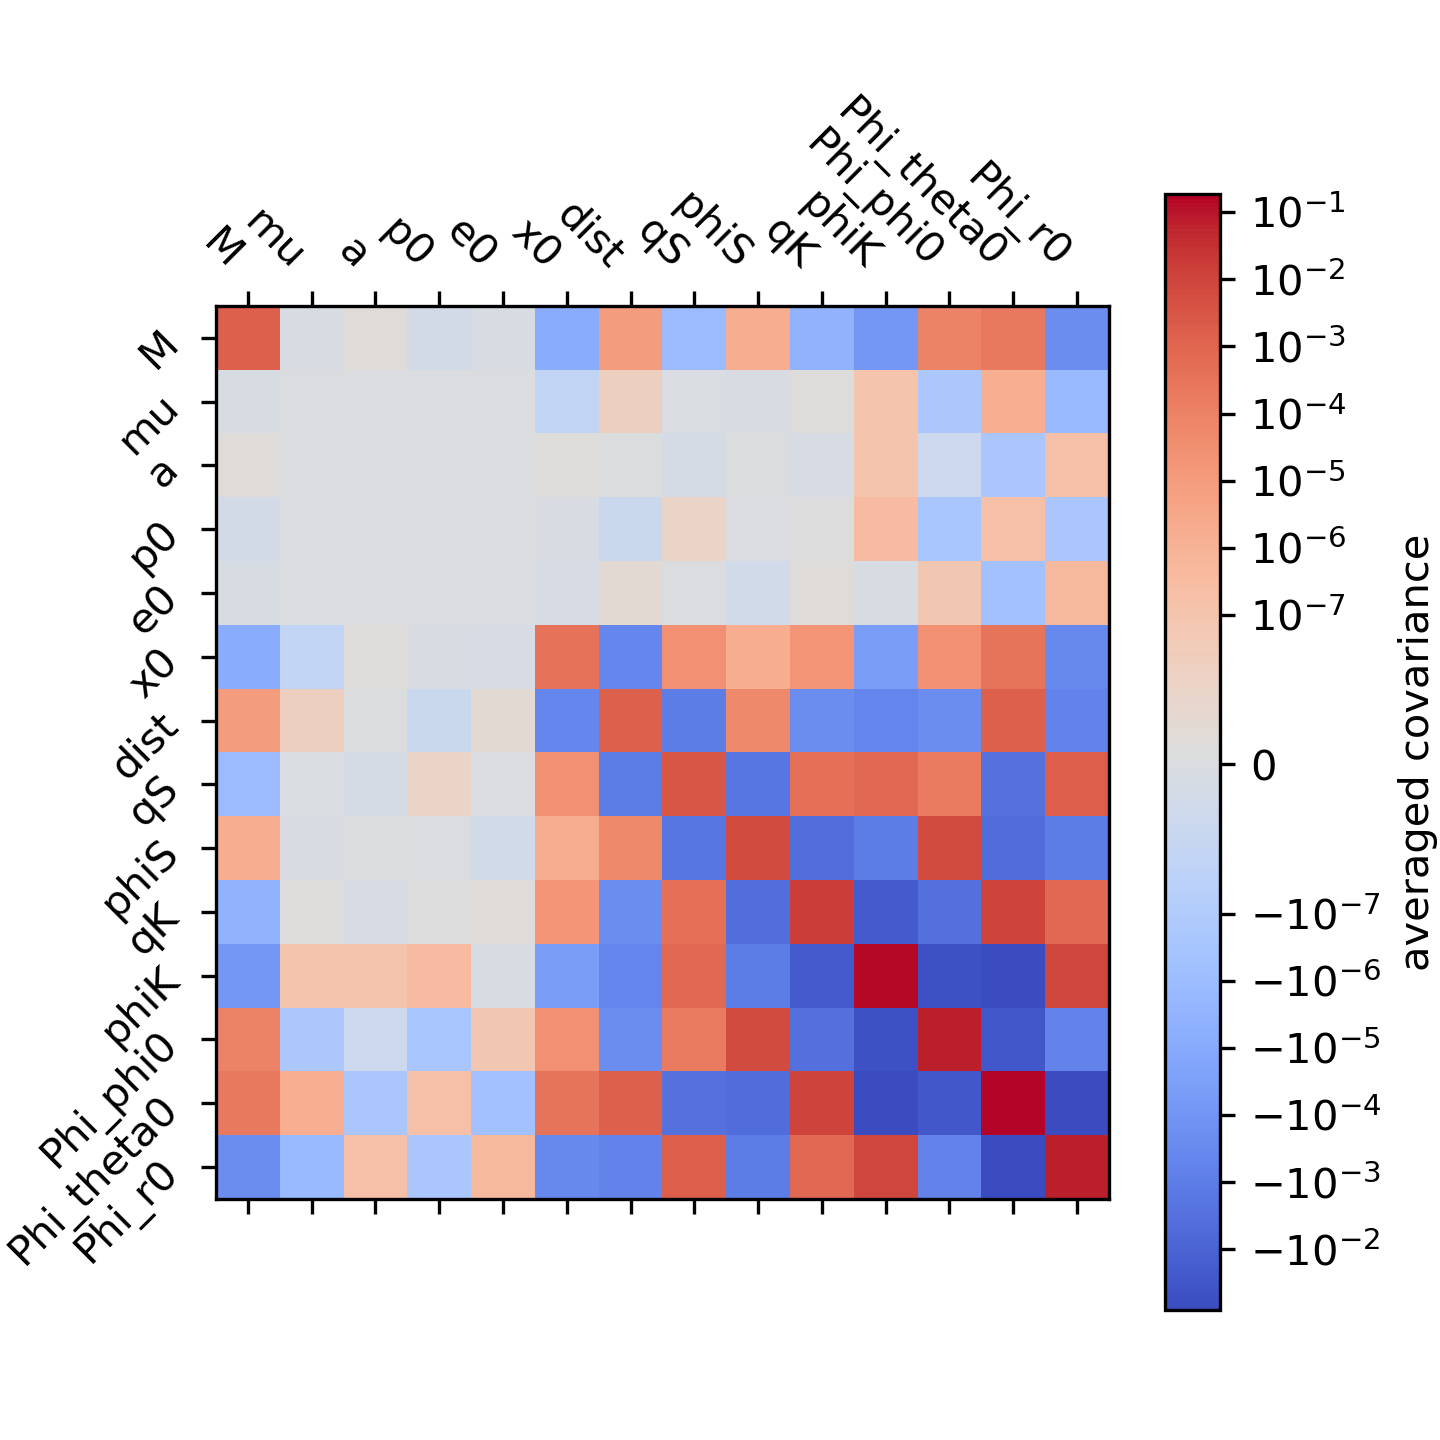
\includegraphics[width=0.8\textwidth]{mean_bounds.png}
    \caption[Average Cramér-Rao bounds]{The average Cramér-Rao bounds for the parameters of the EMRI signal.}
    \label{fig:galaxy-catalog-only-cramer-rao-bounds}
\end{figure}

\begin{figure}
    \centering
    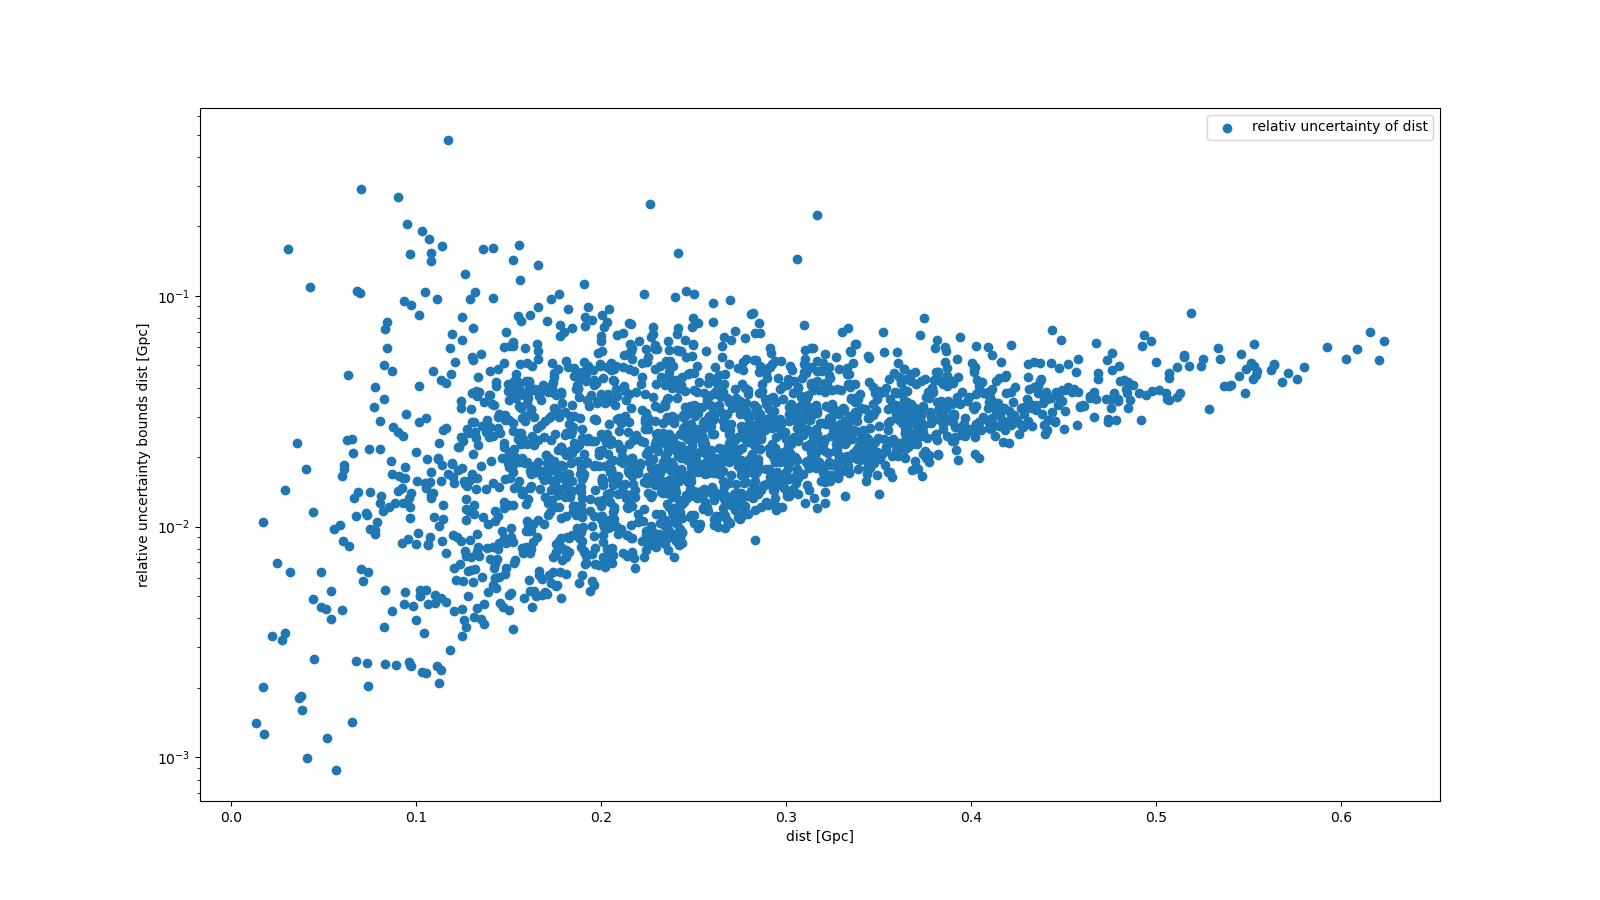
\includegraphics[width=0.8\textwidth]{error_dist.png}
    \caption[Relative luminosity distance uncertainty]{The distribution of the relative luminosity distance uncertainty $\sigma_{\dl} / \dl$ for the simulated detections.}
    \label{fig:rel-luminosity-distance-uncertainty}
\end{figure}

\begin{figure}
    \centering
    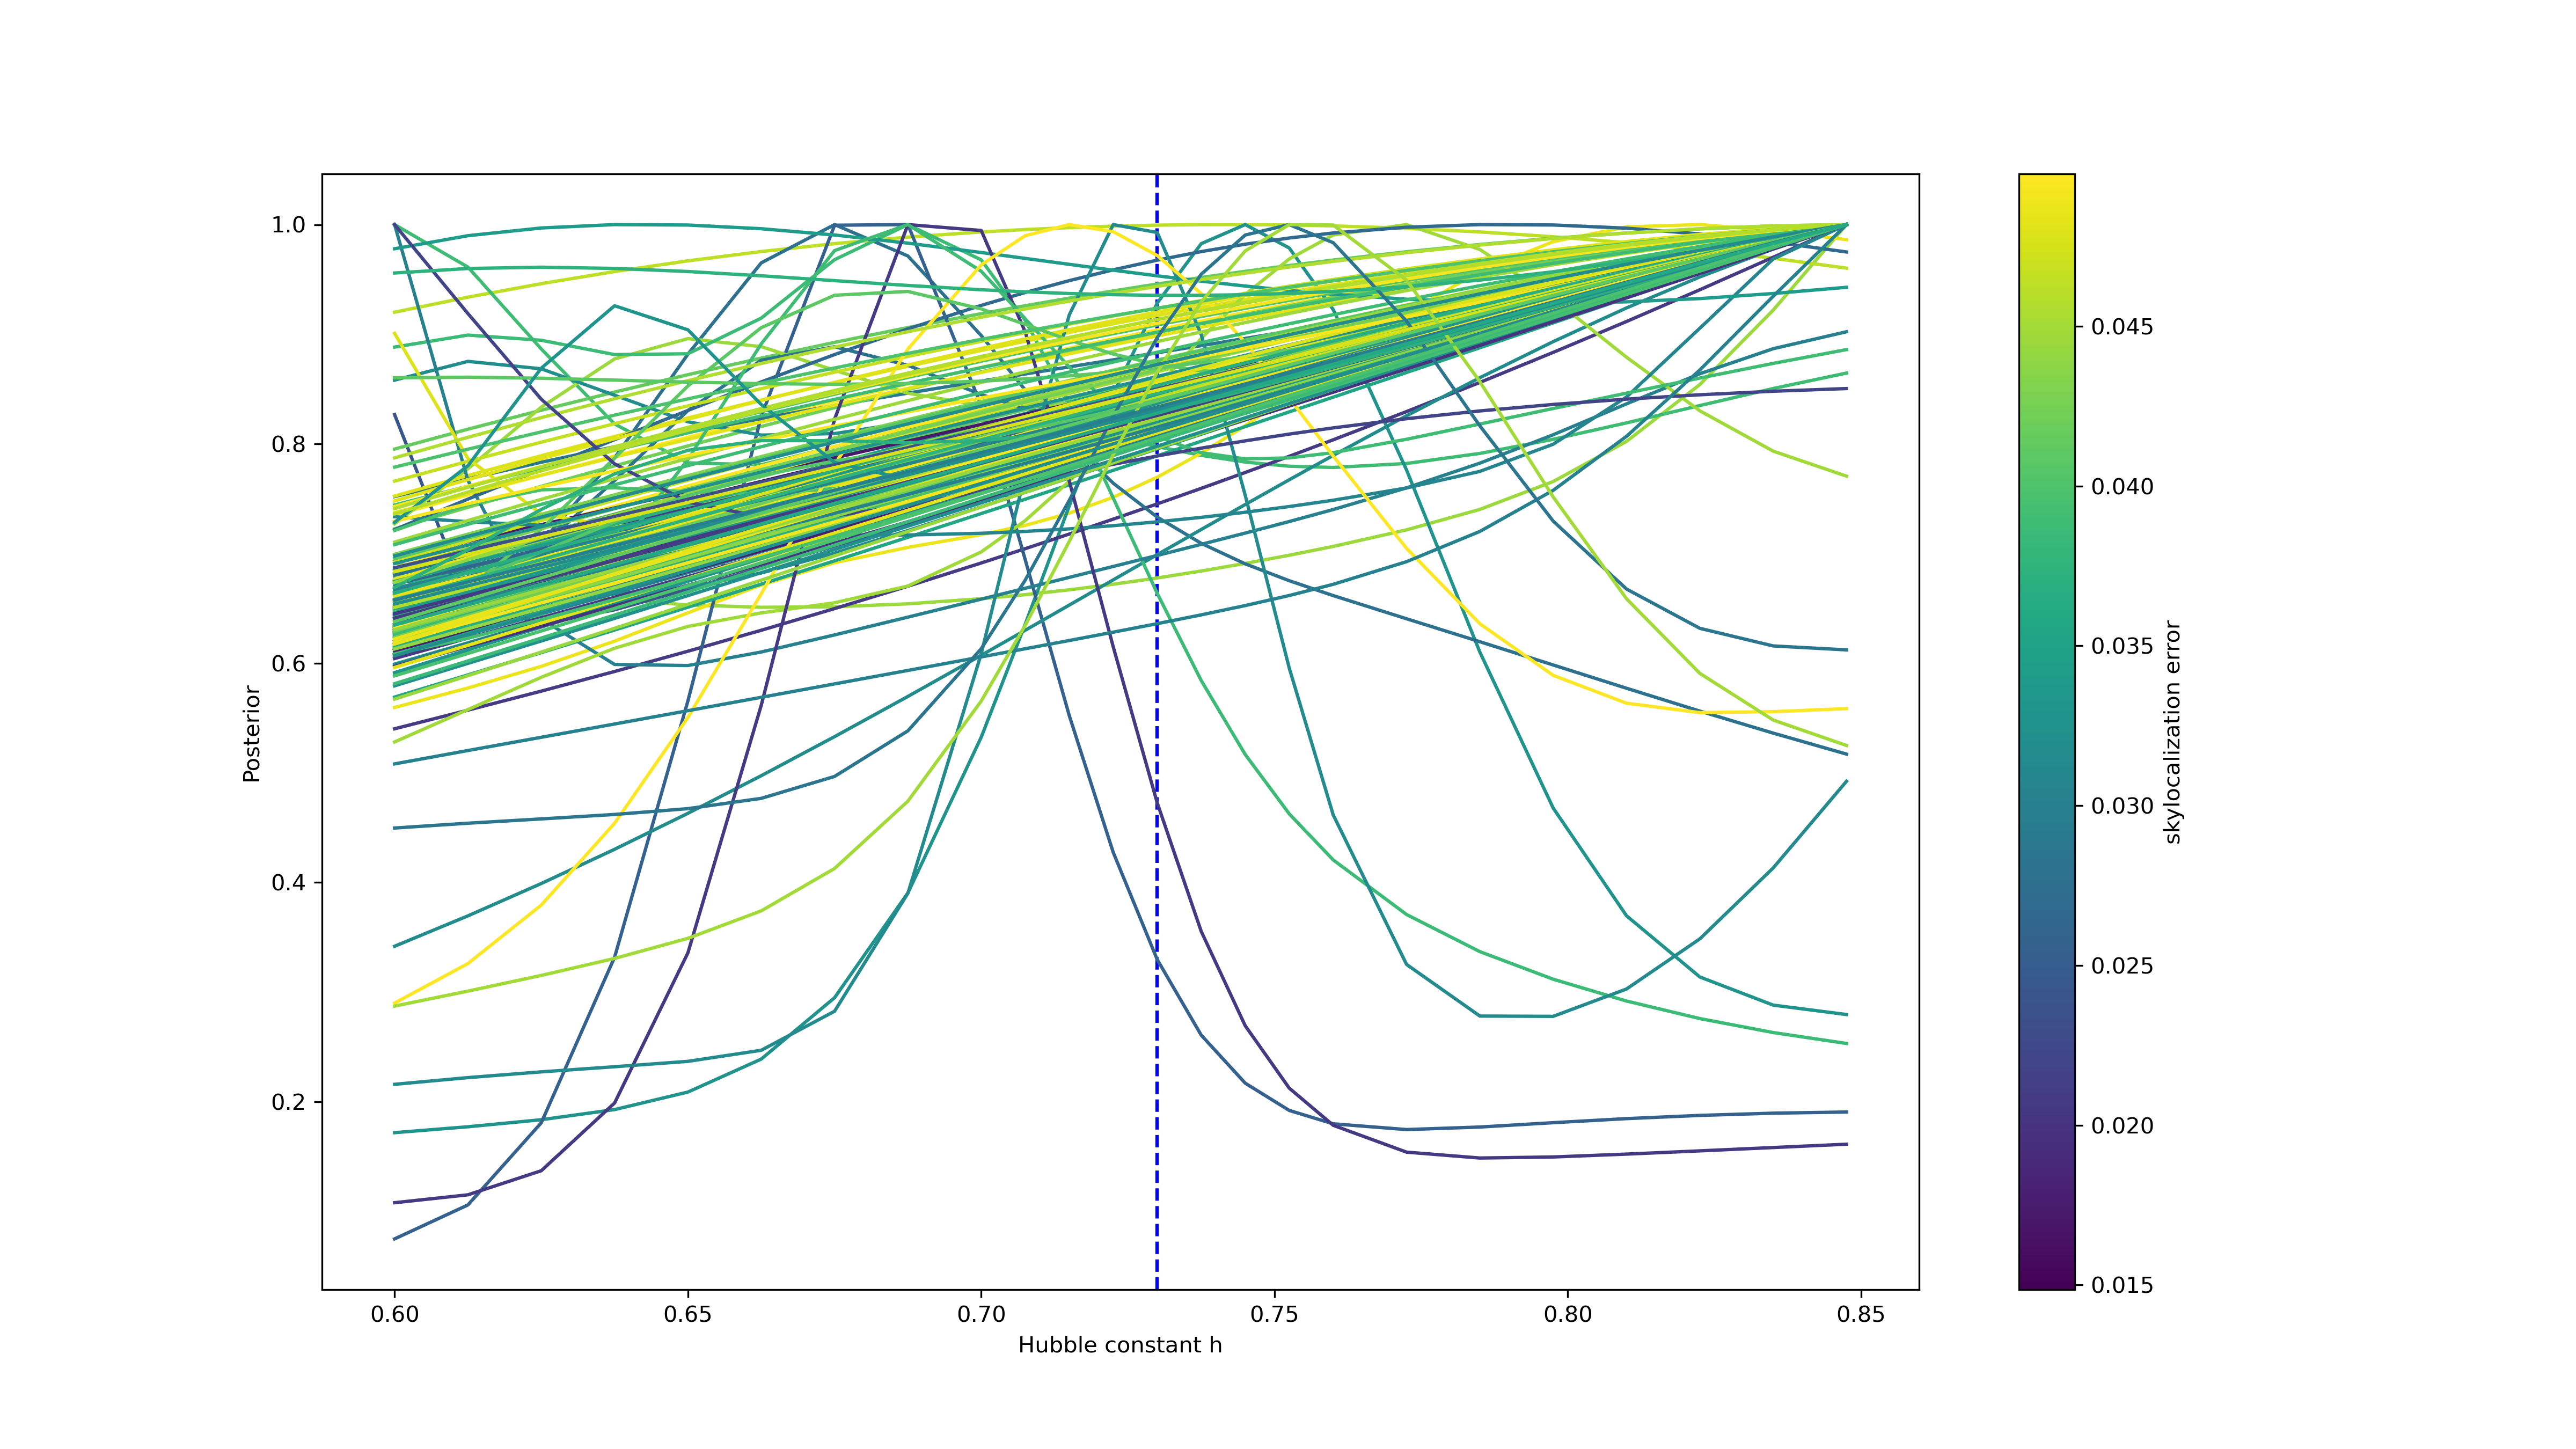
\includegraphics[width=\textwidth]{bayesian_statistics_event_posteriors.png}
    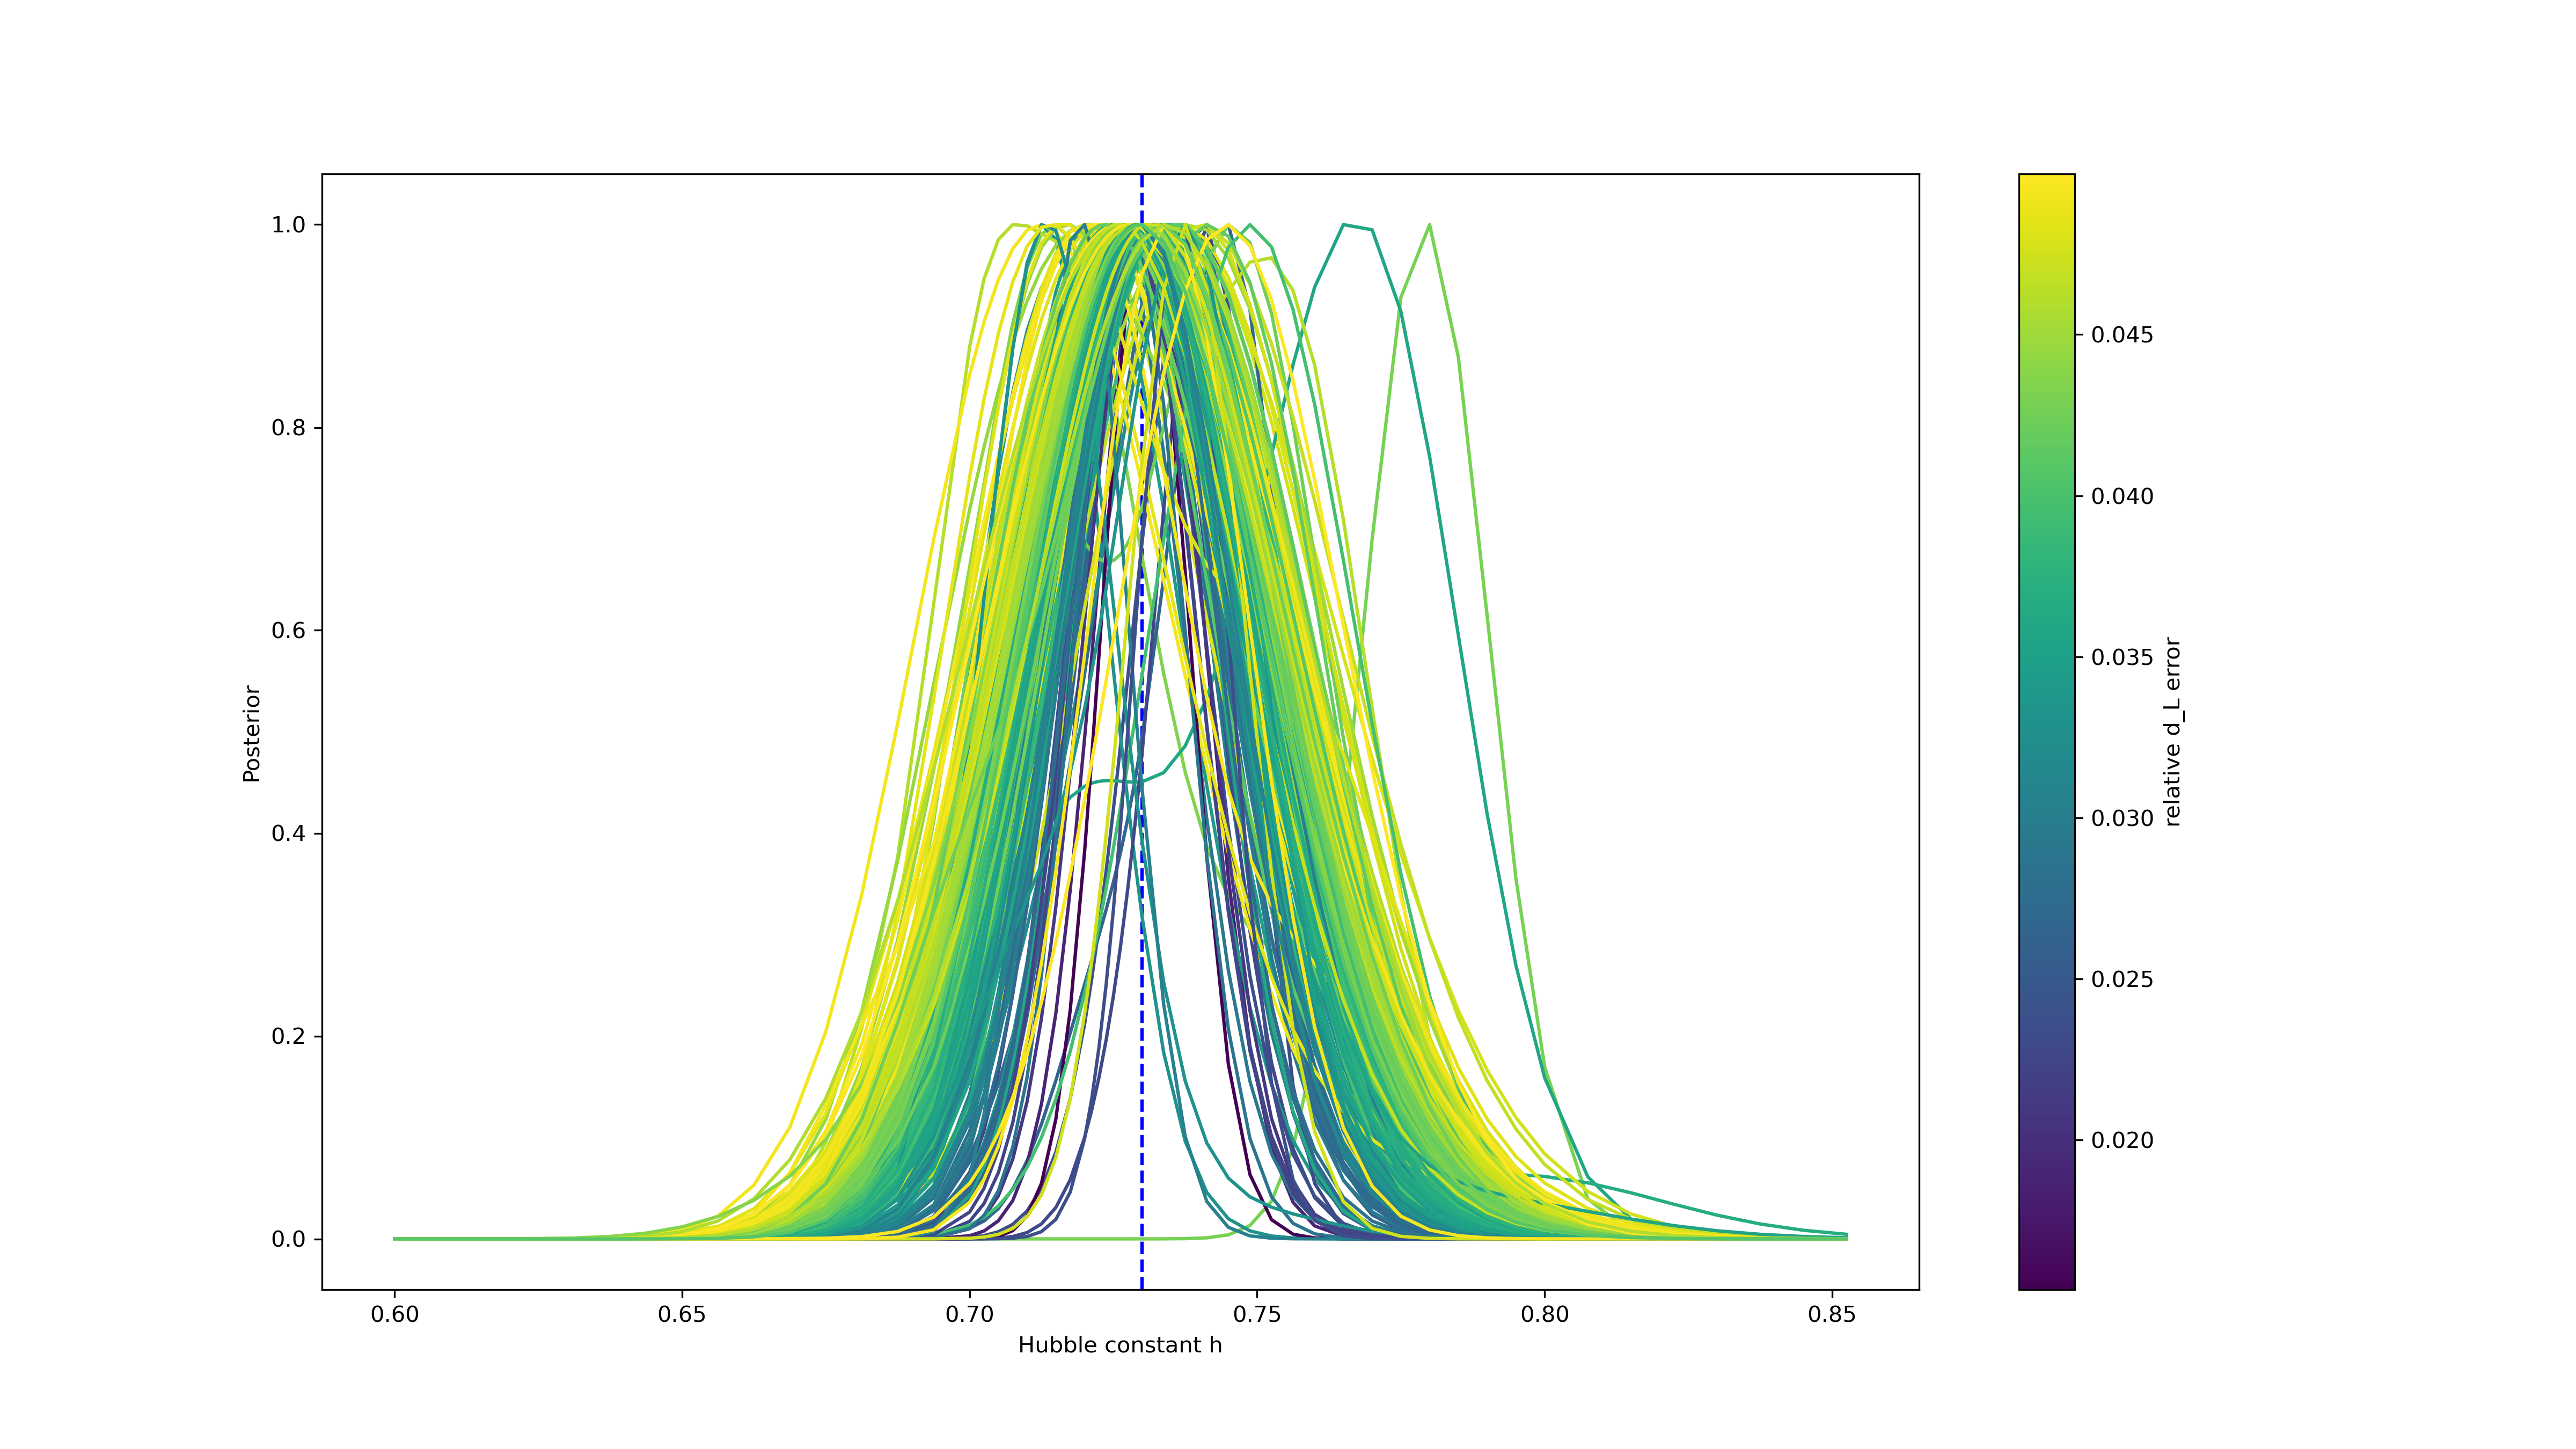
\includegraphics[width=\textwidth]{bayesian_statistics_event_posteriors_with_bh_mass.png}
    \caption[Posterior probability distribution of single detections]{The posterior probability distribution of $\rhubble$ for the single detections without (top) and with (bottom) the usage of the black hole mass $\Mz$ measurement and the galaxy catalog as ground truth. The color indicates the relative luminosity distance uncertainty $\sigma_{\dl} / \dl$. The vertical blue dashed line indicates the true value of $\rhubble = 0.73$.}
    \label{fig:posterior-rhubble-single-detections}
\end{figure}

\begin{figure}
    \centering
    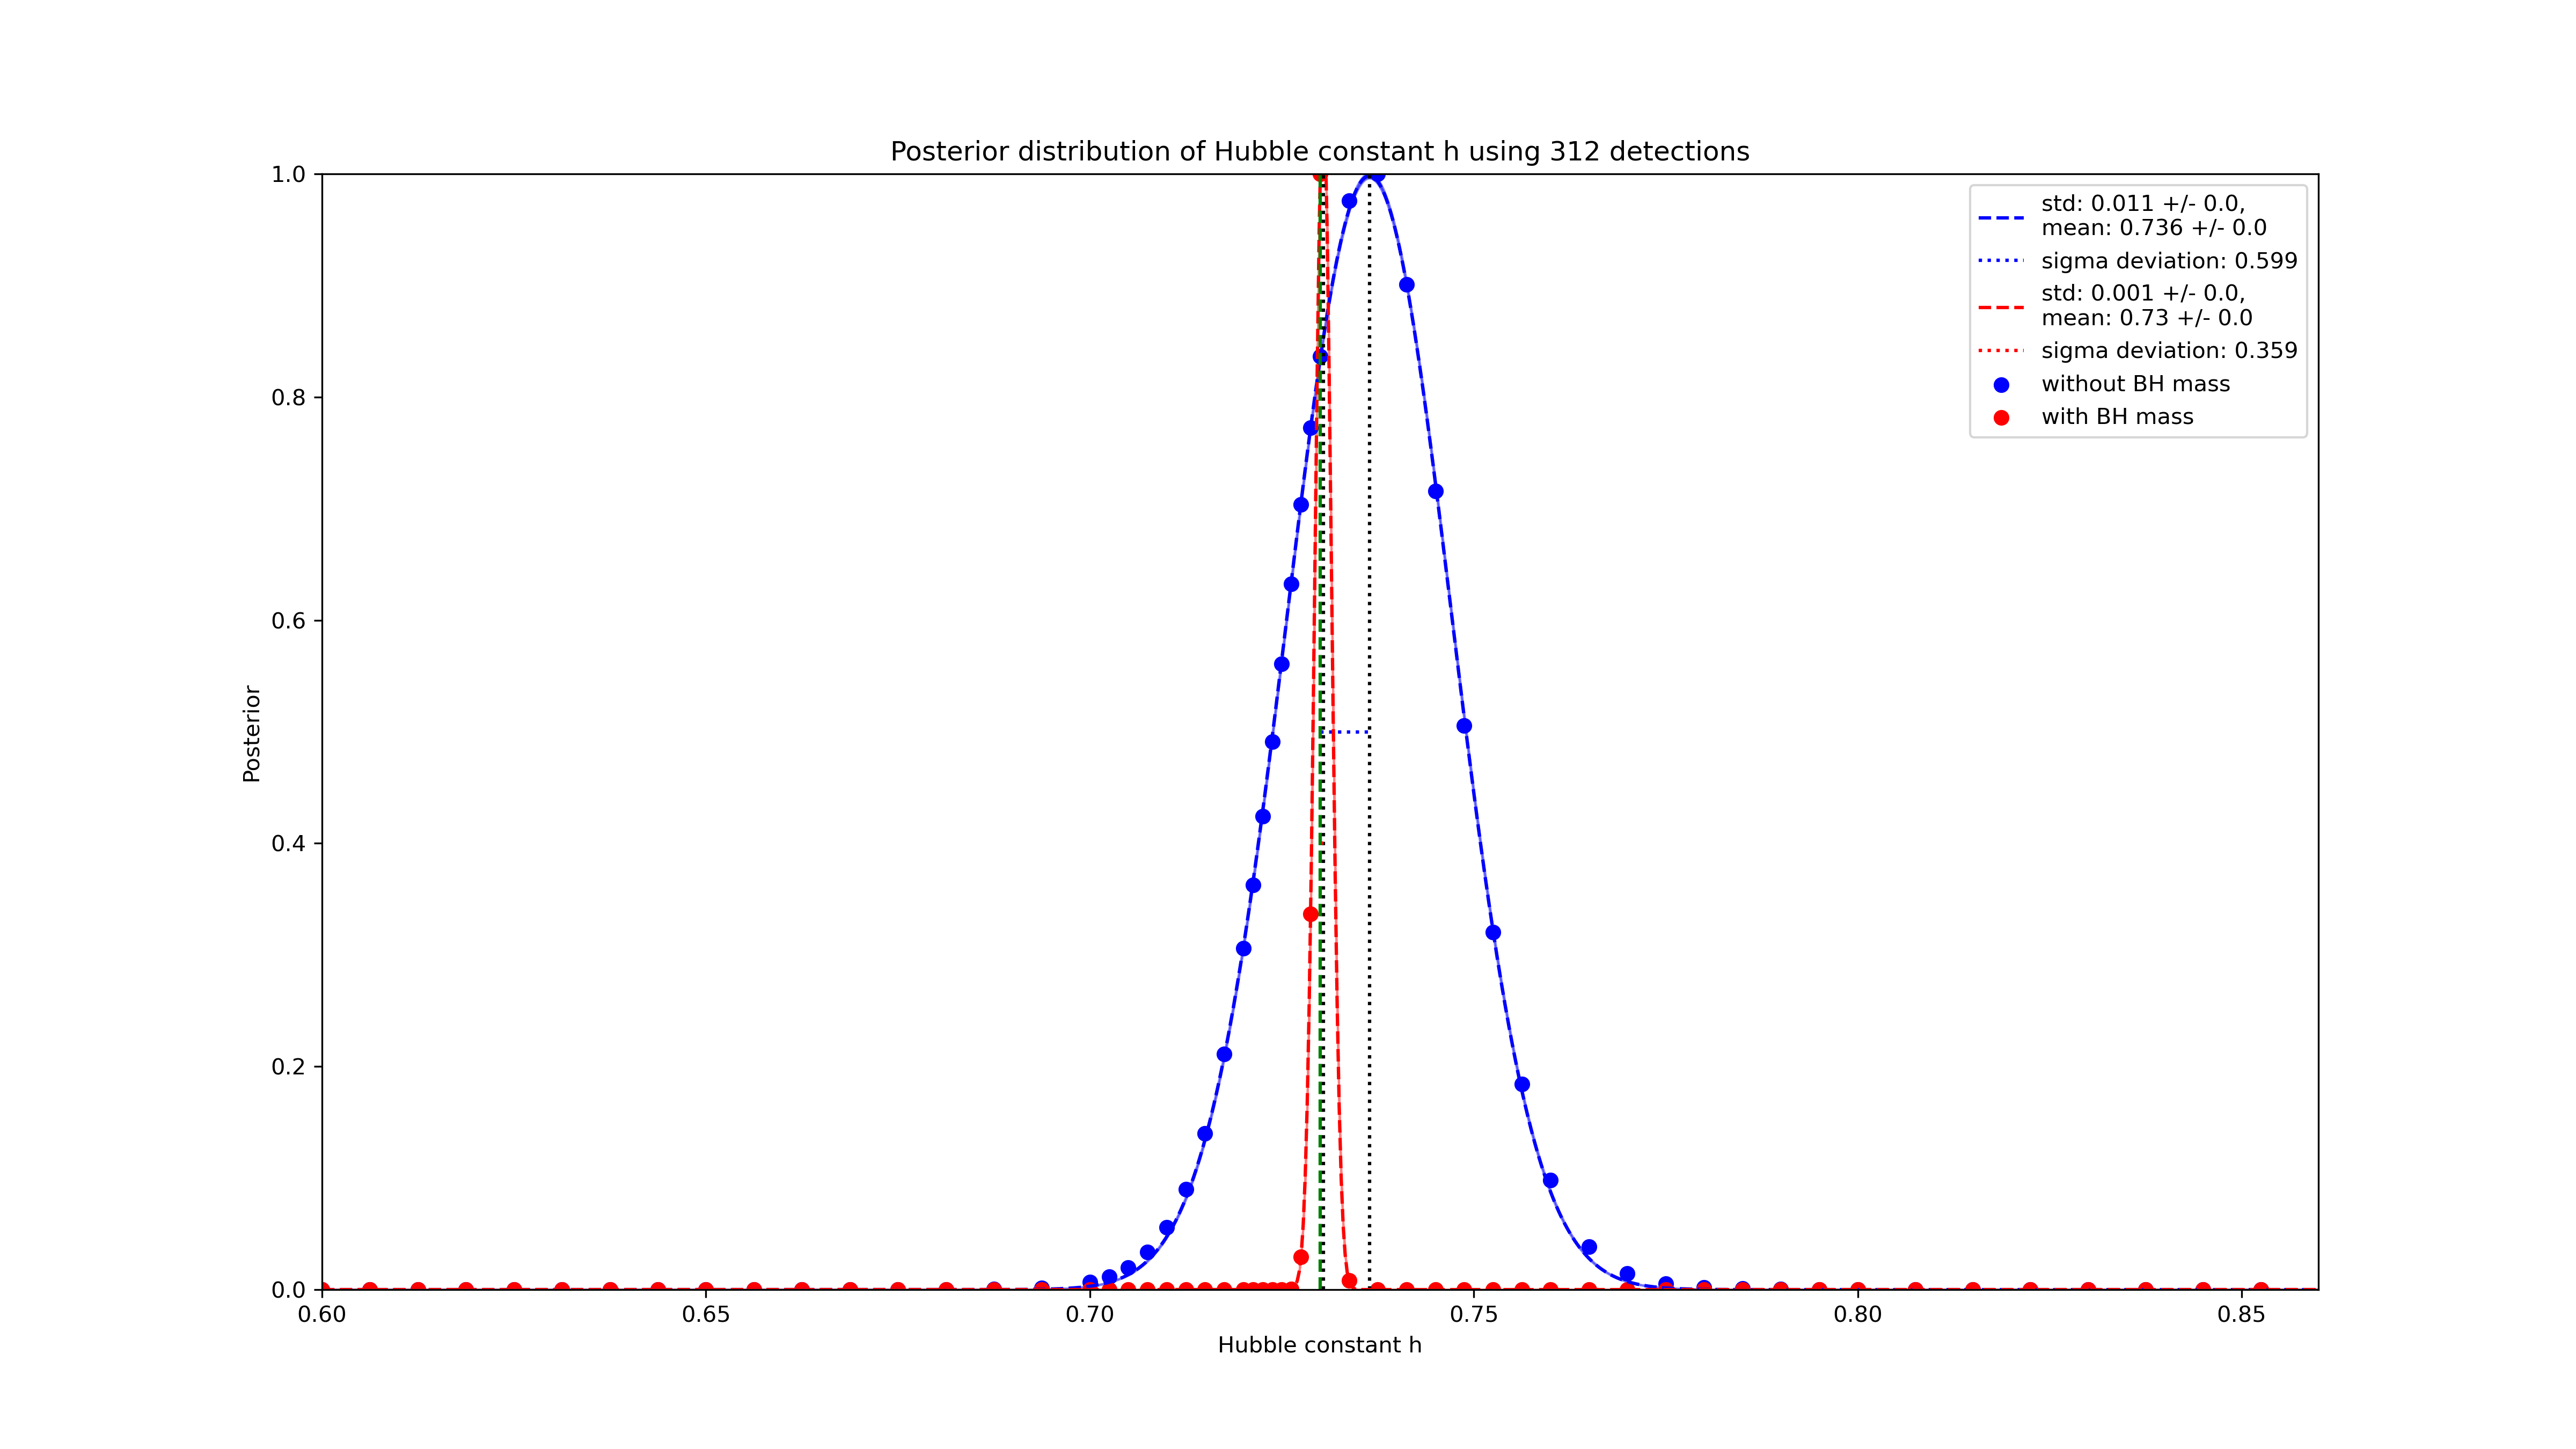
\includegraphics[width=\textwidth]{bayesian_statistics.png}
    \caption[Posterior probability distribution of $\rhubble$]{The posterior probability distribution of $\rhubble$ for the simulated detections with and without using the measured black hole mass $\Mz$.The vertical green dashed line indicates the true value of $\rhubble = 0.73$.}
    \label{fig:posterior-rhubble}
\end{figure}

\begin{figure}
    \centering
    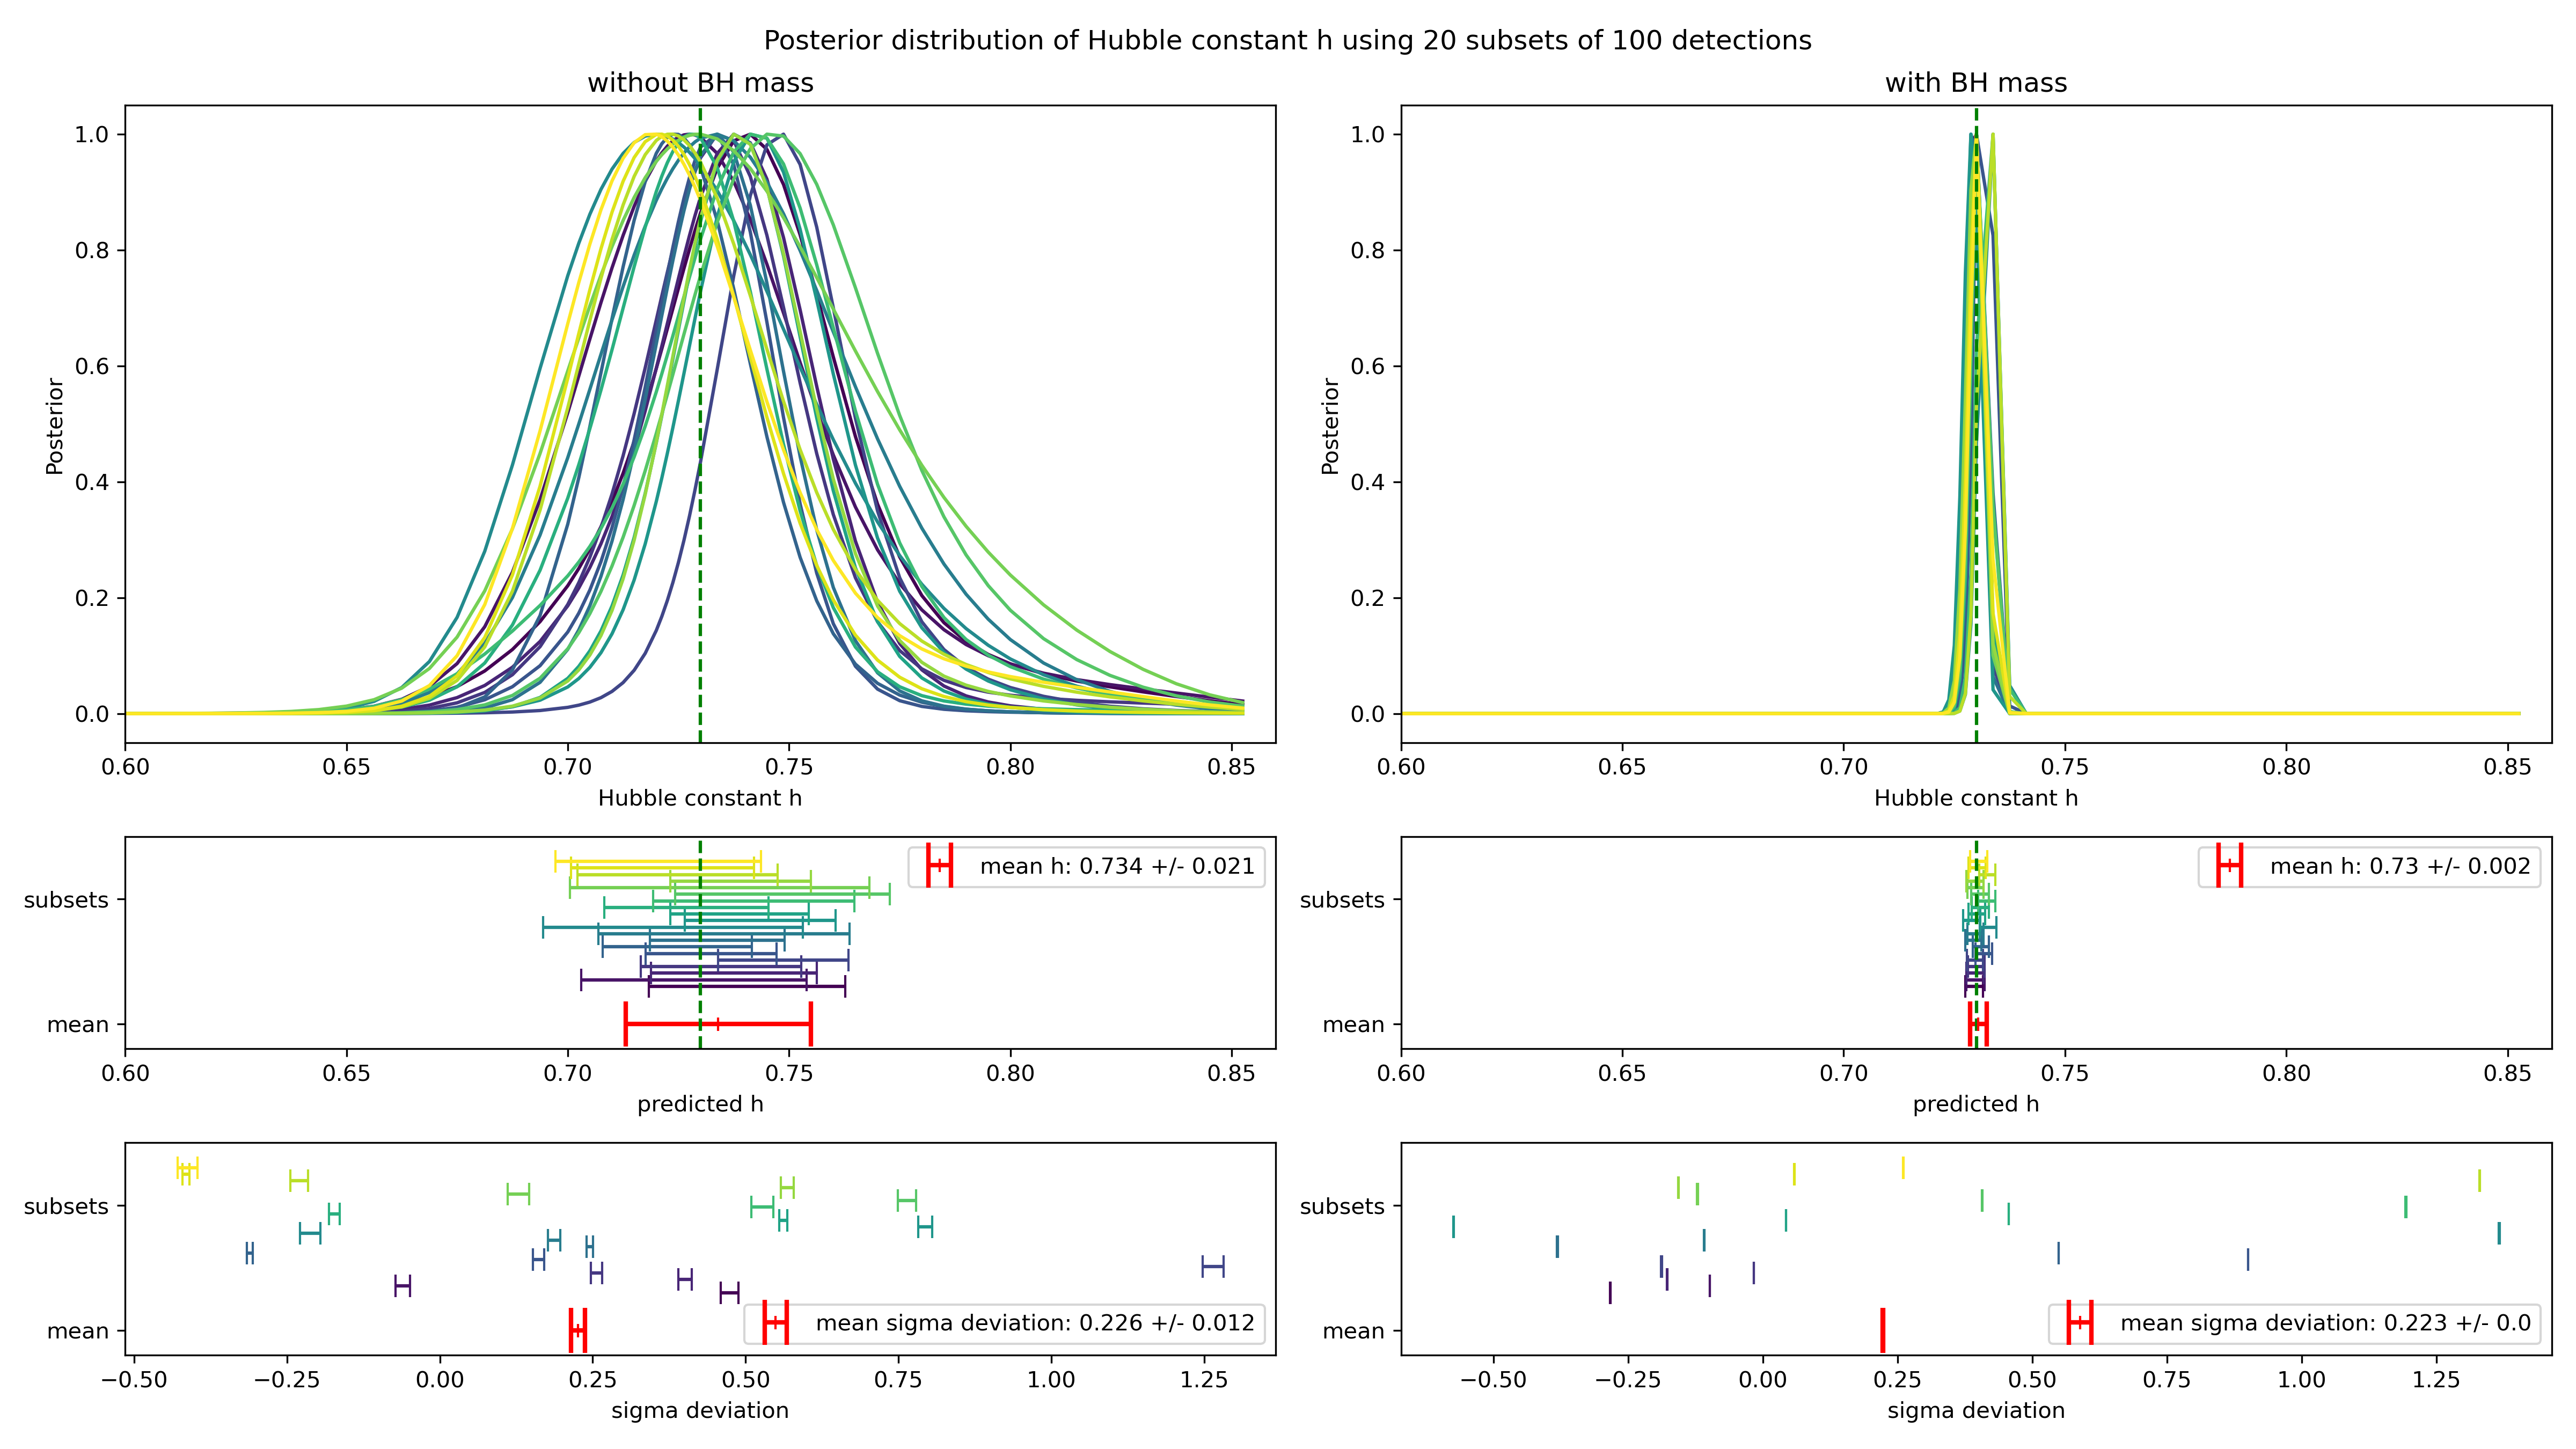
\includegraphics[width=\textwidth]{bayesian_statistics_event_posteriors_subsets.png}
    \caption[Posterior probability distribution of $\rhubble$ of subsets (100 detections)]{The posterior probability distribution of $\rhubble$ for random subsets with 100 detections of the simulated detections with the measured black hole mass $\Mz$. The vertical green dashed line indicates the true value of $\rhubble = 0.73$. The colors indicate the different subsets.}
    \label{fig:posterior-rhubble-subsets}
\end{figure}

\begin{figure}
    \centering
    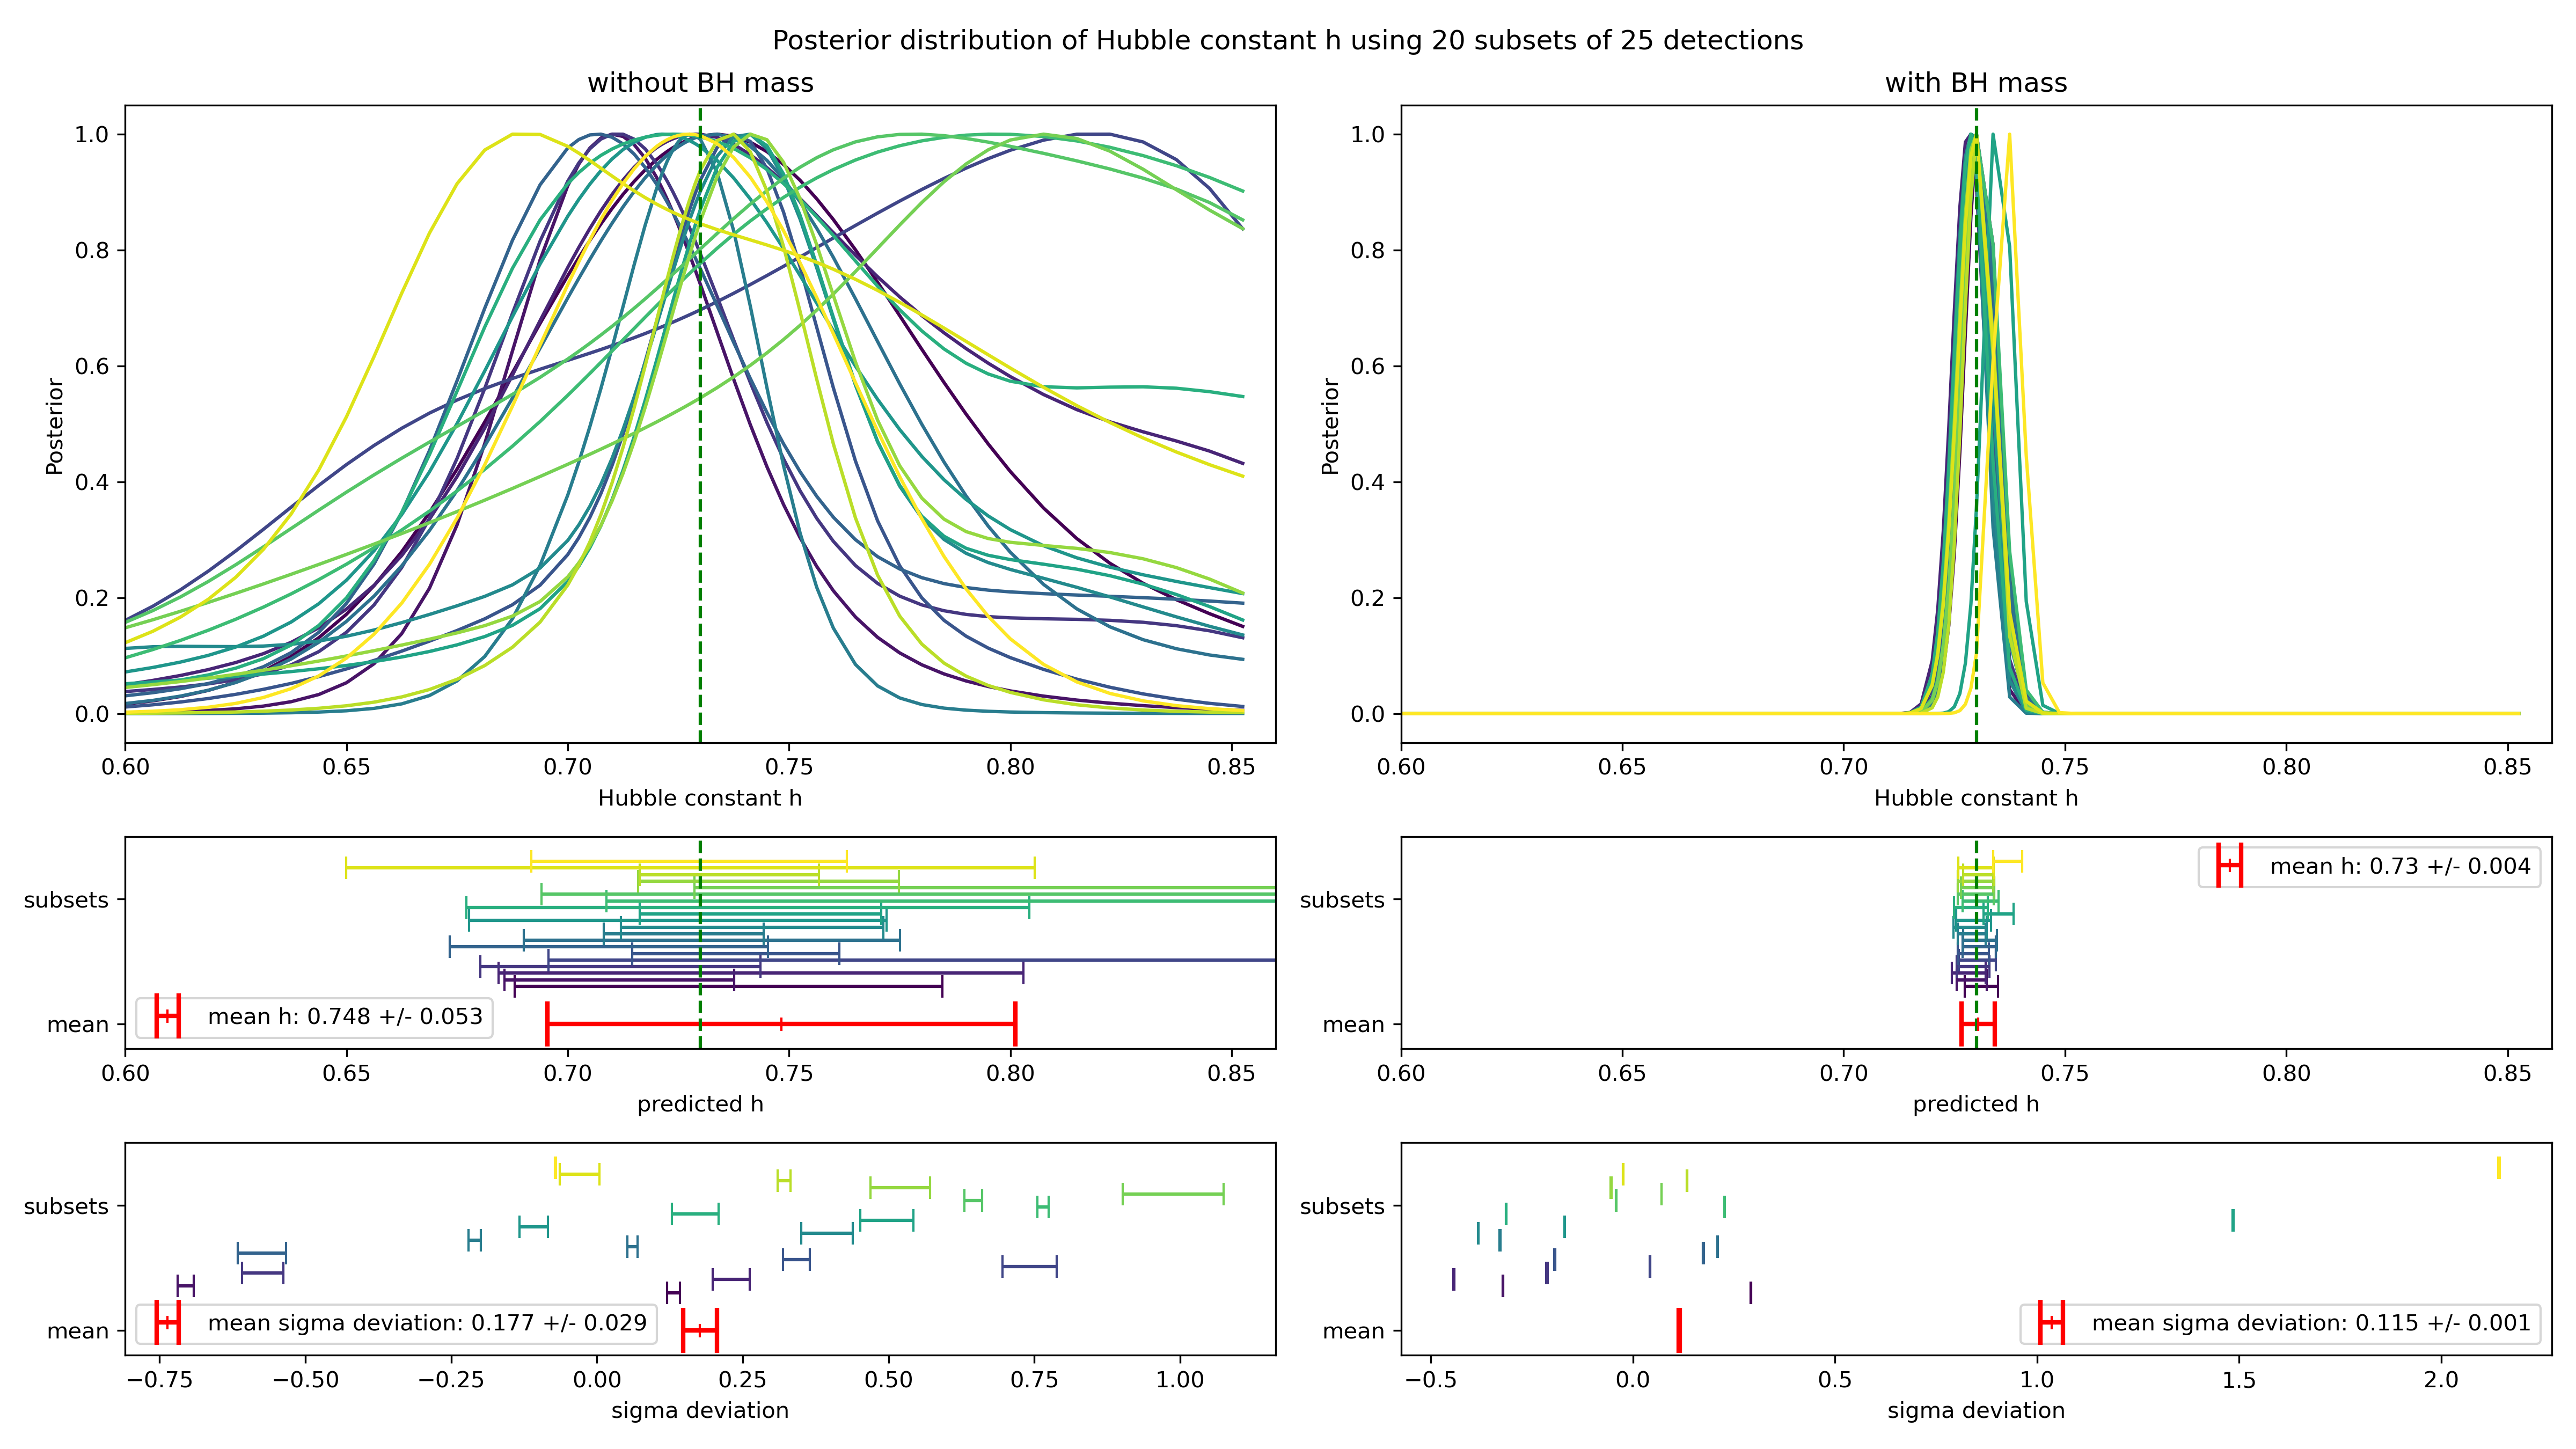
\includegraphics[width=\textwidth]{bayesian_statistics_event_posteriors_subsets_25.png}
    \caption[Posterior probability distribution of $\rhubble$ of subsets (25 detections)]{The posterior probability distribution of $\rhubble$ for random subsets with 25 detections of the simulated detections with the measured black hole mass $\Mz$. The vertical green dashed line indicates the true value of $\rhubble = 0.73$. The colors indicate the different subsets.}
    \label{fig:posterior-rhubble-subsets-25}
\end{figure}
